\section{Parton Distribution Function} \label{sec:higgs:partons}

The LHC collides protons, however looking at the feynman diagrams in
\cref{fig:higgs_production} we see that it is quarks and gluons (a.k.a partons)
that produce these fundamental interactions. This is an indicator that when we
calculate the production cross section for a process at the LHC, we have to not
only consider the hard-scatter probability of the specific diagram, but also
consider the composition of the proton itself.  Specifically, we must consider
the fraction of the total momentum of the proton held by each of its constituent
partons.  This concept is described by Parton Distribution Functions (PDFs)
which give the probability that the indicated parton carries momentum fraction
$x$ of the proton when probed at with energy scale $Q$.  An example PDF for $Q =
10\text{GeV}^2$ and $Q = 10^{4}$GeV in \cref{fig:parton_distribution_function}

\begin{figure}[!htbp]
  \begin{center}
    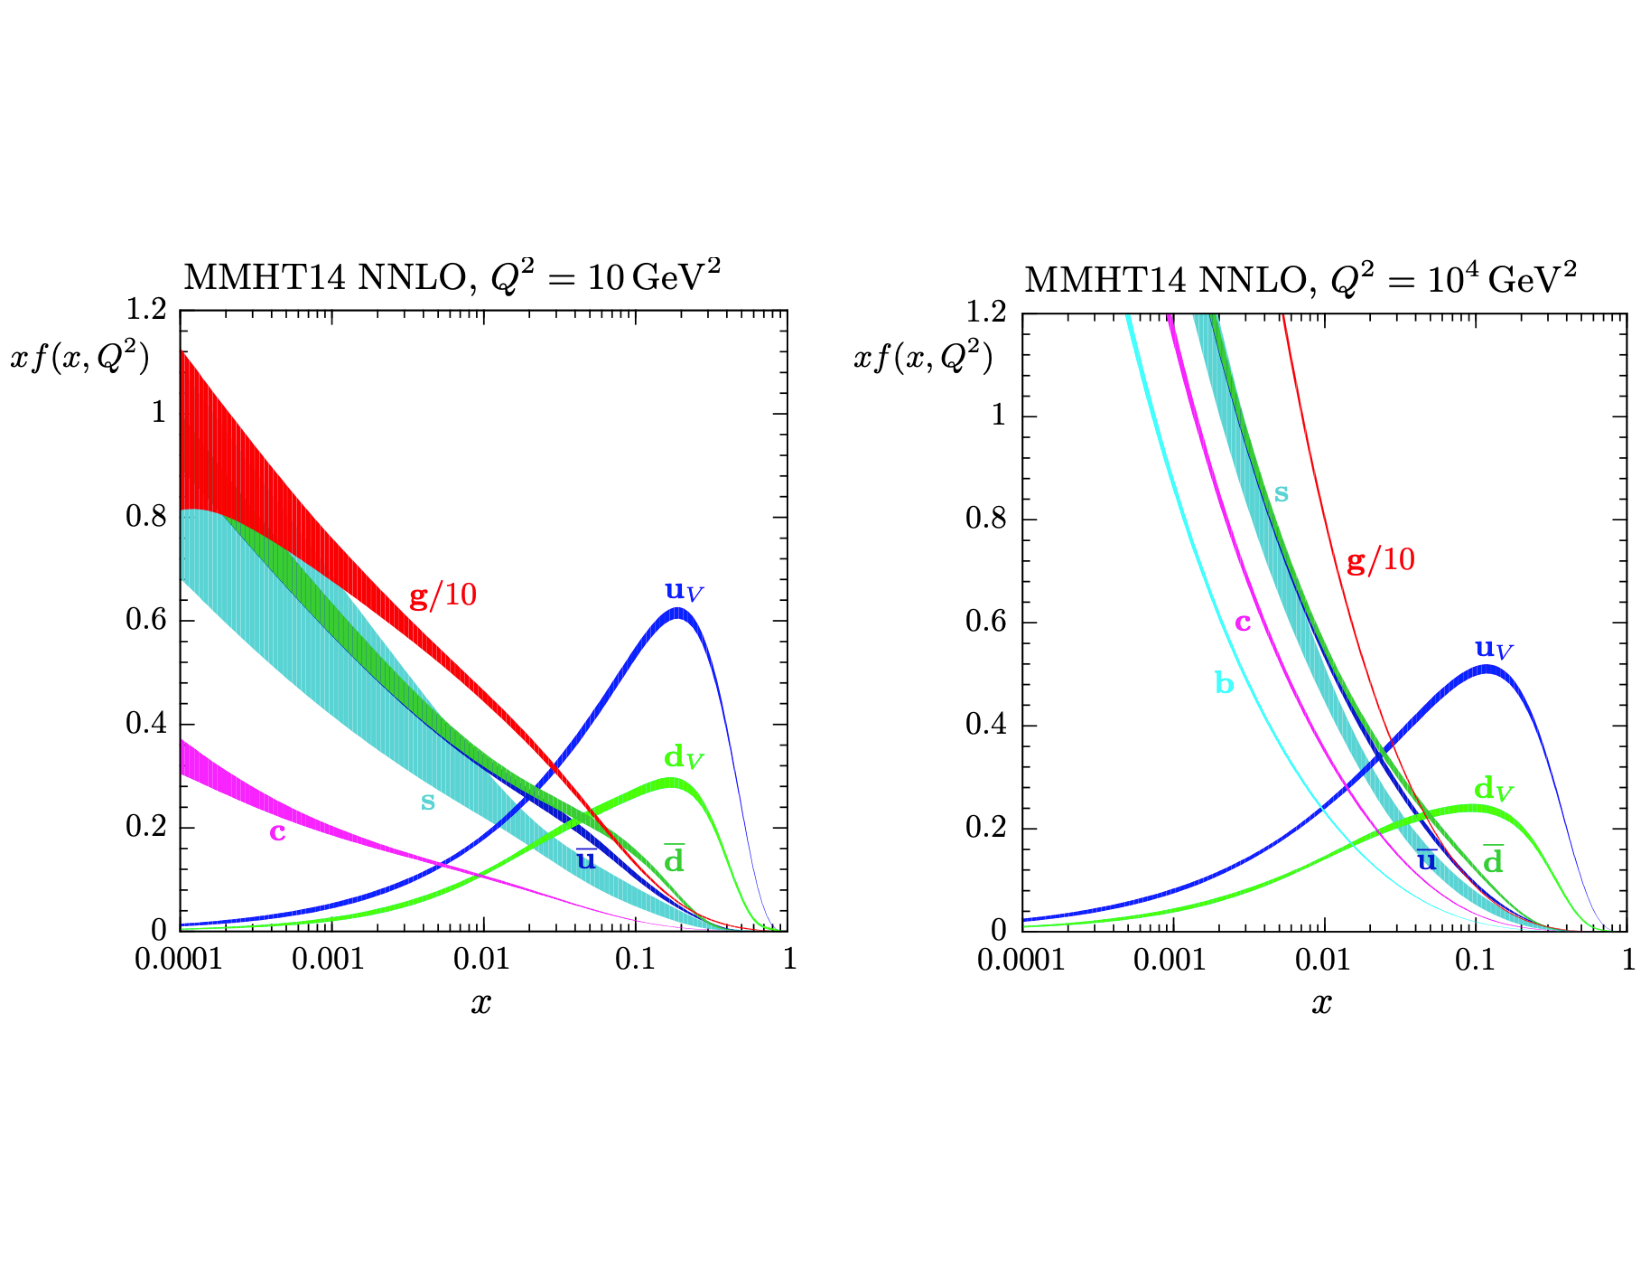
\includegraphics[width=0.8\linewidth]{figures/higgs/pdf.pdf}
    \caption{ \cite{Harland-Lang2015} MMHT2014 NNLO PDFs at $Q2 = 10\text{GeV}^{2}$ and $Q2
=10^{4}\text{GeV}^{2}$ with associated 68\% confidence-level uncertainty bands.
The colored regions indicate the probability of finding the labeled parton with
a momentum fraction given along the x axis. As expected the $u_V$ and $d_V$
contain the largest fraction of the momentum, however we can also see that many
gluons will exist with smaller fractions of the total momentum. Note that as
$Q^2$ increases you are more likely to find something besides a $u/d$}
    \label{fig:parton_distribution_function}
  \end{center}
\end{figure}
